En esta sección se documenta la arquitectura lógica actual del sistema, centrada en la aplicación web, la organización del código y las integraciones externas necesarias para soportar los módulos implementados.

\subsection{Diseño de alto nivel}

KinEstilistas se implementa como una aplicación web monolítica full-stack. La misma base de código contiene tanto la interfaz de usuario como la lógica de servidor y el acceso a datos, lo que simplifica la trazabilidad entre requisitos, código y despliegue.

Los contenedores lógicos que forman la solución son los siguientes:

\begin{itemize}
    \item \textbf{Cliente web}: interfaz renderizada con \texttt{Next.js} y \texttt{React}, diferenciada por rol.
    \item \textbf{Servidor de aplicación}: \texttt{Route Handlers}, autenticación, protección de rutas, validación y orquestación de servicios.
    \item \textbf{Base de datos relacional}: \texttt{PostgreSQL}, persistida y versionada mediante migraciones.
    \item \textbf{Servicios externos}: \texttt{Cloudinary} para imágenes, \texttt{Nominatim} para geocodificación y \texttt{OSRM} para trazado de rutas.
\end{itemize}

La aplicación resuelve además varias responsabilidades transversales desde una capa común:

\begin{itemize}
    \item autenticación y sesión con \texttt{Auth.js},
    \item control de acceso por rol,
    \item compatibilidad mínima de navegador,
    \item rate limiting sobre \texttt{/api},
    \item contratos de datos compartidos entre cliente y servidor.
\end{itemize}

\subsection{Diseño detallado}

La estructura del código combina una organización por capas técnicas con subdirectorios funcionales para las áreas principales del dominio.

\begin{itemize}
    \item \texttt{app/admin/}, \texttt{app/commercials/} y \texttt{app/clients/}: entrada funcional por rol.
    \item \texttt{app/api/}: endpoints internos segmentados por área de negocio.
    \item \texttt{app/components/}: componentes de interfaz reutilizables, incluyendo formularios, mapas y tablas.
    \item \texttt{app/hooks/api/}: capa cliente para acceso declarativo a la API.
    \item \texttt{lib/contracts/}: DTOs y contratos comunes.
    \item \texttt{lib/commercial/}: lógica de planificación de rutas y cálculo temporal reutilizable.
    \item \texttt{lib/typeorm/entities/} y \texttt{lib/typeorm/services/}: modelo persistente y servicios de dominio asociados a la base de datos.
    \item \texttt{migrations/typeorm/}: evolución versionada del esquema.
\end{itemize}

\paragraph{Flujo típico de una operación protegida}

El flujo interno de una operación sensible sigue de forma general los siguientes pasos:

\begin{enumerate}
    \item La petición llega a \texttt{proxy.ts}, donde se aplica control de navegador, autenticación base y rate limiting.
    \item La página o el endpoint correspondiente obtiene la sesión y comprueba el rol requerido.
    \item El \textit{Route Handler} delega la lógica de negocio en servicios o helpers de \texttt{lib/}.
    \item Si se requiere persistencia, la operación utiliza \texttt{TypeORM} sobre entidades y repositorios.
    \item La respuesta se normaliza y se devuelve al cliente mediante contratos compartidos.
\end{enumerate}

\paragraph{Organización actual por carpetas}

La arquitectura de carpetas actual es adecuada para el alcance ya construido, porque separa claramente:

\begin{itemize}
    \item vistas por rol,
    \item componentes visuales reutilizables,
    \item integraciones externas,
    \item persistencia y migraciones.
\end{itemize}

No obstante, el crecimiento del módulo comercial ya apunta a una evolución deseable: reforzar la agrupación por \textit{feature} para reducir la dispersión entre componentes, hooks, contratos y servicios relacionados con una misma capacidad de negocio. La base actual sigue siendo válida, pero esta mejora será especialmente interesante cuando entren en alcance \texttt{M3} y \texttt{M4}.

\subsection{Gestión de almacenamiento de imágenes de perfil}
\label{sec:storageDesign}
En el estado actual del proyecto, el almacenamiento del sistema se divide en tres categorías complementarias: datos estructurados persistentes, activos multimedia externos y datos operativos derivados bajo demanda.

\subsubsection*{Datos estructurados persistentes}

La información principal del dominio se almacena en \texttt{PostgreSQL} mediante entidades gestionadas con \texttt{TypeORM} \citep{postgresdocs2026,typeormentities2026}. Esto incluye:

\begin{itemize}
    \item usuarios, solicitudes de alta, accesos y trazabilidad administrativa;
    \item clientes, comerciales y asignaciones entre ambos;
    \item visitas, rutas comerciales y ordenacion de paradas;
    \item estructura de catálogo, productos, cartas de color y referencias cromáticas;
    \item pedidos, líneas de pedido, estados de negocio y estado mínimo de cobro;
    \item fichas técnicas del salón, servicios, plantillas, productos utilizados, sugerencias e imágenes finales referenciadas;
    \item segmentos de cliente, asignaciones comerciales de segmentación, promociones, formaciones, inscripciones, notificaciones internas y recordatorios;
    \item catálogos controlados de roles, estados y tipos operativos utilizados por los módulos ya implementados;
    \item sobrescrituras técnicas persistidas para políticas de rate limiting;
    \item configuraciones del sistema, integraciones externas, operaciones de integración y propuestas de pedido a proveedor con sus líneas.
\end{itemize}

Este modelo relacional actúa como fuente de verdad del sistema. Las operaciones críticas de autenticación, gestión comercial, catálogo, pedidos, administración transversal y operación empresarial se apoyan en esta capa. La Figura~\ref{fig:postgresql-physical-model} recoge el diseño físico completo de PostgreSQL.

\begin{figure}[H]
    \centering
    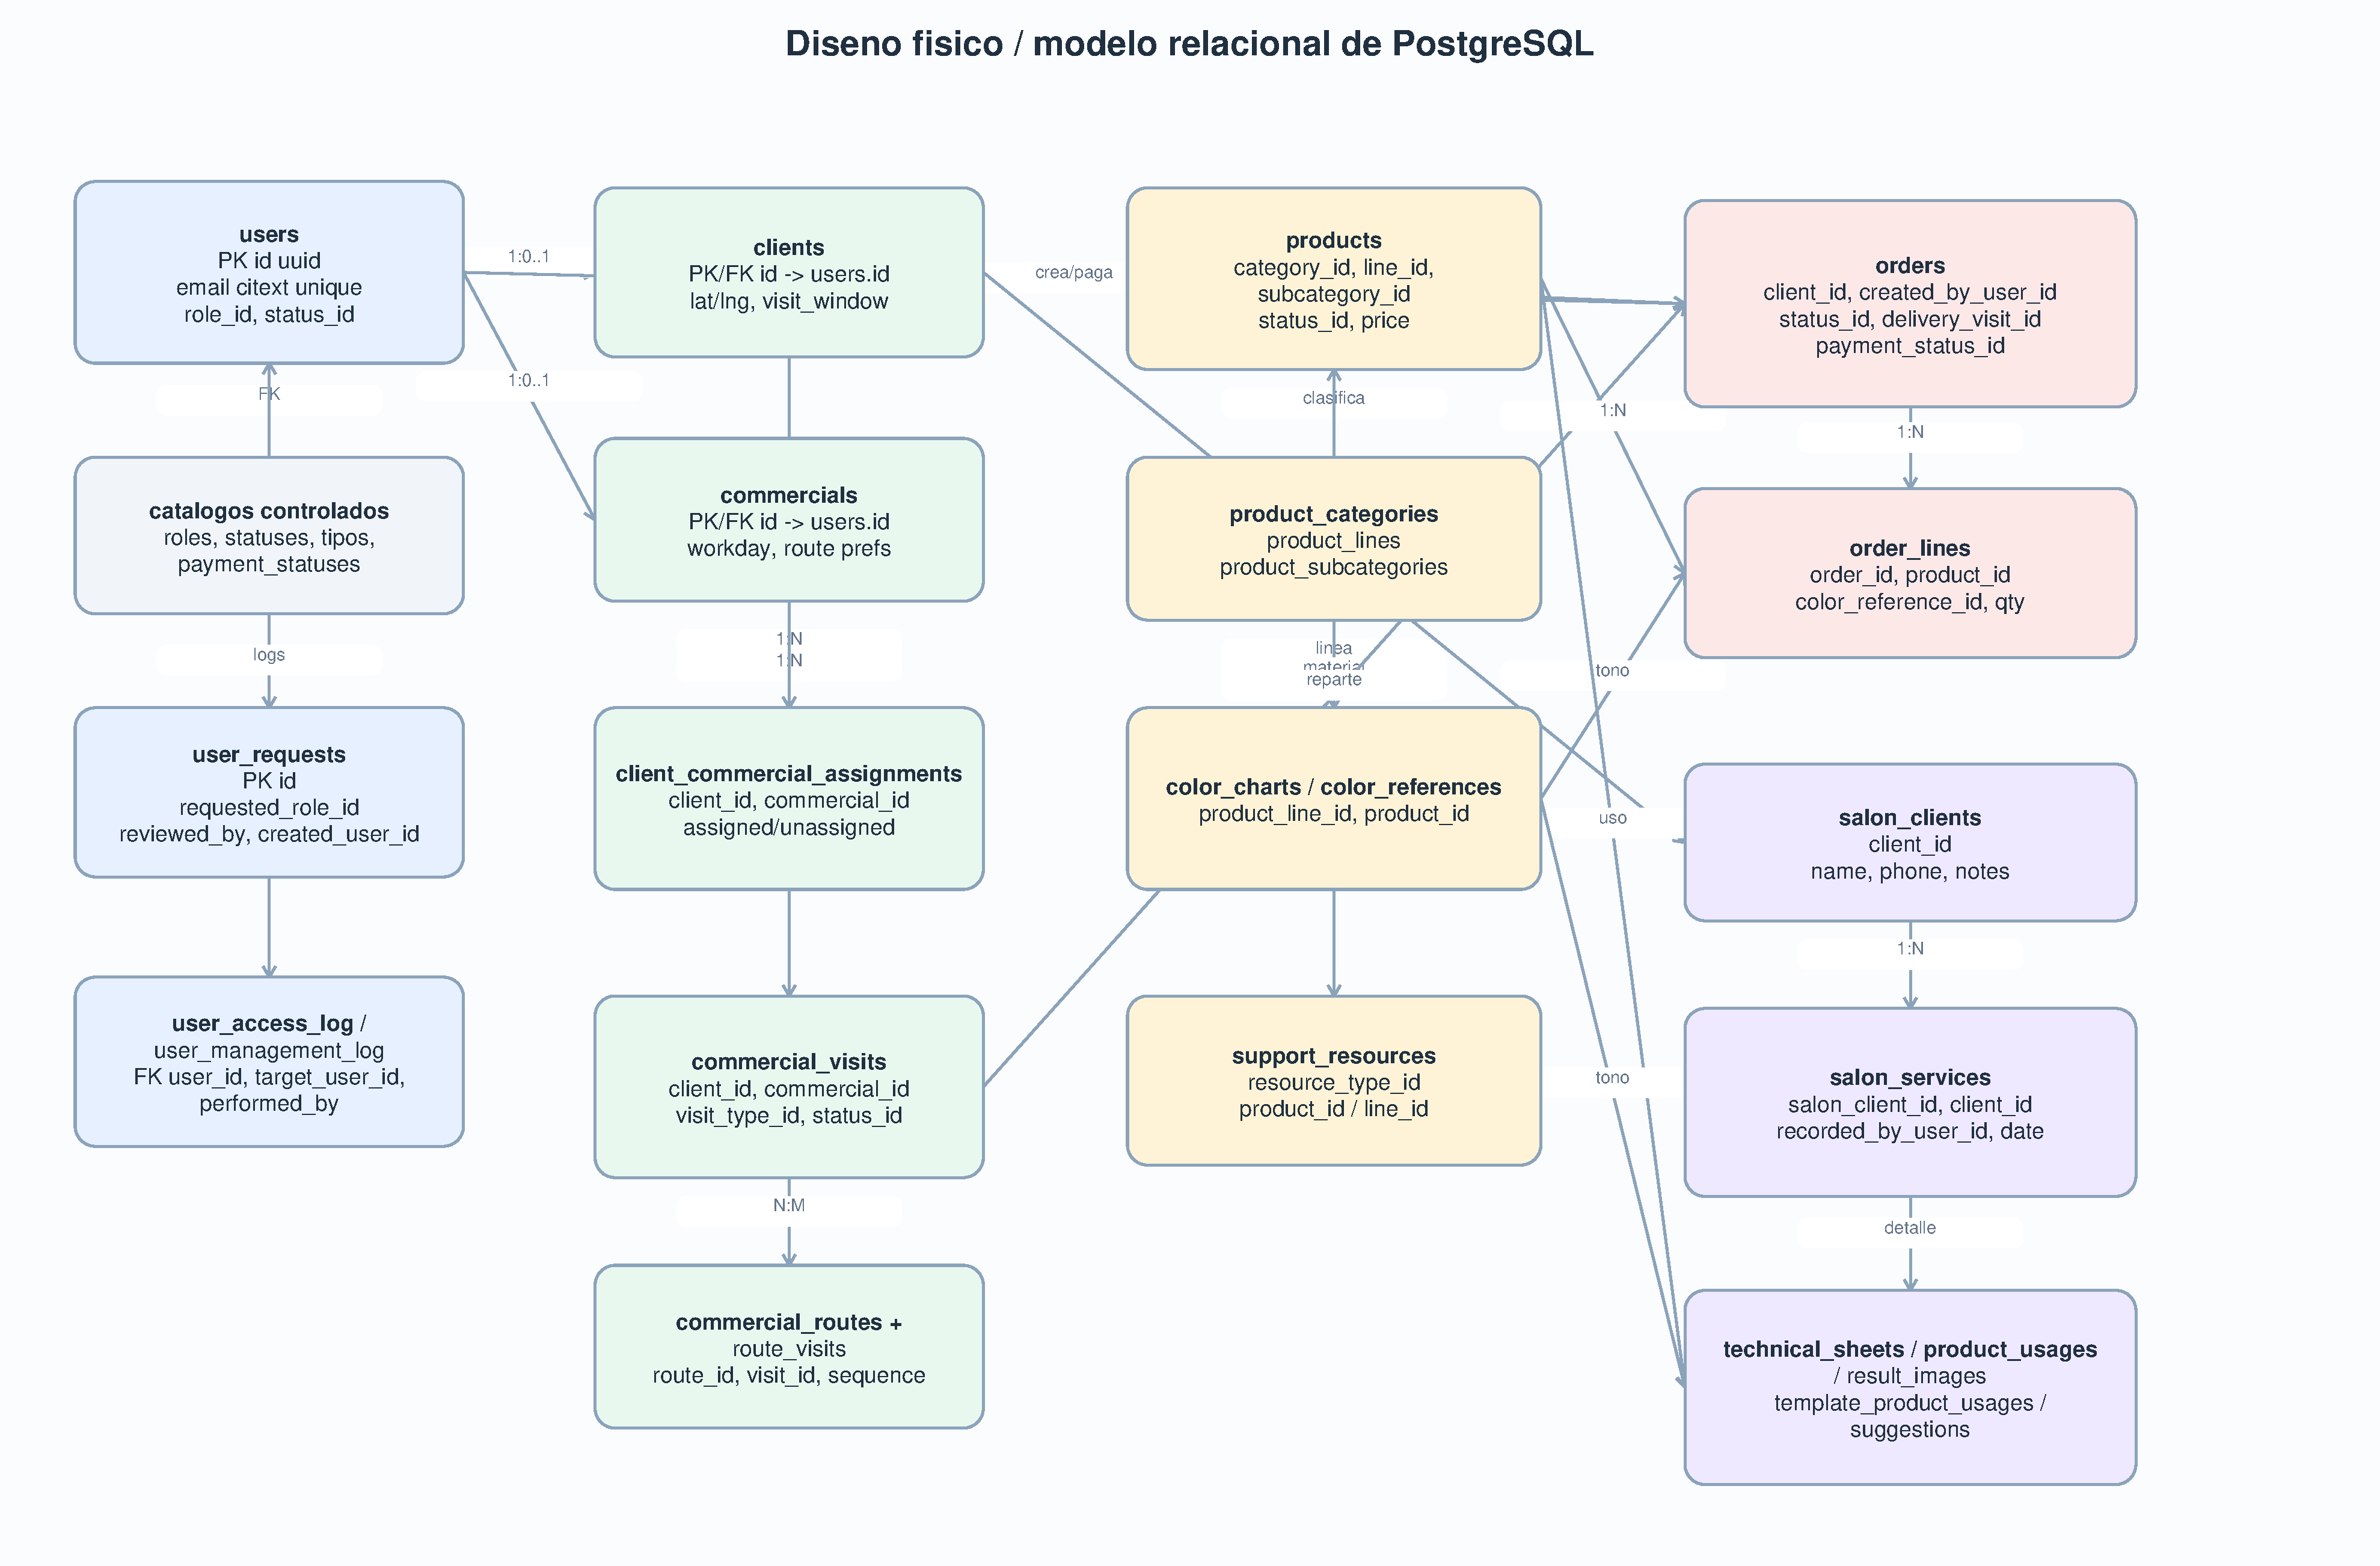
\includegraphics[width=\linewidth]{./figures/UML/MCD/postgresql-physical-model.pdf}
    \caption{Diseño físico / modelo relacional de PostgreSQL}
    \label{fig:postgresql-physical-model}
\end{figure}

\subsubsection*{Activos multimedia externos}

Las imágenes no se almacenan como binarios en la base de datos. En su lugar, la aplicación delega su gestión en \texttt{Cloudinary} \citep{cloudinaryupload2026}. Esta decisión afecta actualmente a dos familias de activos:

\begin{itemize}
    \item imágenes de perfil de usuarios;
    \item imágenes de catálogo, incluyendo líneas, subcategorías, productos, cartas de color y referencias cromáticas;
    \item imágenes del resultado final de servicios técnicos registrados en el salón.
\end{itemize}

En la base de datos solo se persisten las URLs finales y, cuando procede, metadatos auxiliares como la miniatura asociada a una referencia cromática. Esto simplifica el modelo, reduce el peso de la base de datos y permite reutilizar un almacenamiento optimizado para contenido multimedia.

\subsubsection*{Datos derivados o reconstruibles}

Existen además varios artefactos que la aplicación no persiste como entidad independiente:

\begin{itemize}
    \item el QR del pedido, que se reconstruye a partir del identificador del pedido y se representa mediante \texttt{QuickChart} \citep{quickchartqr2026};
    \item la geometría de ruta comercial, que se consulta a \texttt{OSRM} en tiempo de ejecución \citep{osrmdocs2026};
    \item la geocodificación de una dirección, que se obtiene desde \texttt{Nominatim} cuando hace falta confirmar o recalcular coordenadas \citep{nominatimapi2026};
    \item la ETA visible para cliente, que se calcula a partir de visitas reales, reglas horarias y posición en ruta, y no como un dato fijo aislado.
\end{itemize}

Esta separación evita almacenar resultados efímeros o fácilmente regenerables cuando su valor depende de datos del negocio ya presentes en el sistema.

\subsubsection*{Criterios de diseño adoptados}

La estrategia de almacenamiento aplicada en el proyecto responde a cuatro criterios:

\begin{itemize}
    \item mantener el dato estructurado y transaccional dentro de la base de datos relacional;
    \item externalizar los binarios y recursos multimedia a un servicio especializado;
    \item recalcular bajo demanda la información derivada cuando sea más robusto que persistirla;
    \item limitar el número de entidades persistentes a las que realmente aportan valor al modelo de negocio implementado.
\end{itemize}

Por ello, aunque el sistema ya muestra QR, ETA, mapas, capturas de cámara o recursos externos, no todo ello debe interpretarse como nuevas entidades almacenadas. La memoria debe distinguir entre datos persistidos, activos referenciados e información operativa calculada en el momento.

